\chapter*{Лабораторная работа 5. Анализатор сетевого трафика Wireshark}
\addcontentsline{toc}{chapter}{Лабораторная работа 5. Анализатор сетевого трафика Wireshark}

\textbf{Цель работы:} Знакомство с возможностями анализатора сетевого трафика Wireshark.

\section*{1. Установка}
\addcontentsline{toc}{section}{1. Установка}

Для использования \texttt{wireshark} в графическом режиме, потребуется пакет \texttt{wireshark-qt}.
\begin{Verbatim}[frame=single,breaklines=true,breakanywhere=true]
    smart@thinkpad$ sudo pacman -S wireshark-qt
    resolving dependencies...
    looking for conflicting packages...

    Packages (10) bcg729-1.1.1-1  c-ares-1.19.0-1  cdparanoia-10.2-8
                gst-plugins-base-1.22.0-3  libmaxminddb-1.7.1-1
                qt5-multimedia-5.15.8+kde+r2-1  sbc-2.0-1  spandsp-0.0.6-4
                wireshark-cli-4.0.3-1  wireshark-qt-4.0.3-1

    Total Download Size:    28.58 MiB
    Total Installed Size:  138.16 MiB

    :: Proceed with installation? [Y/n] 
    :: Retrieving packages...
    spandsp-0.0.6-4-...   424.1 KiB  1820 KiB/s 00:00 [######################] 100%
    qt5-multimedia-5...   763.0 KiB  2.79 MiB/s 00:00 [######################] 100%
    c-ares-1.19.0-1-...   205.7 KiB  5.02 MiB/s 00:00 [######################] 100%
    sbc-2.0-1-x86_64       47.9 KiB  1197 KiB/s 00:00 [######################] 100%
    bcg729-1.1.1-1-x...    37.6 KiB   939 KiB/s 00:00 [######################] 100%
    libmaxminddb-1.7...    23.9 KiB  1193 KiB/s 00:00 [######################] 100%
    gst-plugins-base...   316.3 KiB   703 KiB/s 00:00 [######################] 100%
    wireshark-qt-4.0...     4.1 MiB  2.56 MiB/s 00:02 [######################] 100%
    wireshark-cli-4.0.3-1-x86_64                                                                                       22.7 MiB  3.37 MiB/s 00:07 [########################################################################################] 100%
    Total (9/9)                                                                                                        28.6 MiB  4.21 MiB/s 00:07 [########################################################################################] 100%
    (10/10) checking keys in keyring                                                                                                               [########################################################################################] 100%
    (10/10) checking package integrity                                                                                                             [########################################################################################] 100%
    (10/10) loading package files                                                                                                                  [########################################################################################] 100%
    (10/10) checking for file conflicts                                                                                                            [########################################################################################] 100%
    (10/10) checking available disk space                                                                                                          [########################################################################################] 100%
    :: Processing package changes...
    ( 1/10) installing cdparanoia                                                                                                                  [########################################################################################] 100%
    ( 2/10) installing gst-plugins-base                                                                                                            [########################################################################################] 100%
    ( 3/10) installing qt5-multimedia                                                                                                              [########################################################################################] 100%
    Optional dependencies for qt5-multimedia
        qt5-declarative: QML bindings [installed]
        gst-plugins-good: camera support, additional plugins
        gst-plugins-bad: camera support, additional plugins
        gst-plugins-ugly: additional plugins
        gst-libav: ffmpeg plugin
    ( 4/10) installing c-ares                                                                                                                      [########################################################################################] 100%
    ( 5/10) installing libmaxminddb                                                                                                                [########################################################################################] 100%
    Optional dependencies for libmaxminddb
        geoip2-database: IP geolocation databases
    ( 6/10) installing spandsp                                                                                                                     [########################################################################################] 100%
    ( 7/10) installing sbc                                                                                                                         [########################################################################################] 100%
    ( 8/10) installing bcg729                                                                                                                      [########################################################################################] 100%
    ( 9/10) installing wireshark-cli                                                                                                               [########################################################################################] 100%
    NOTE: To run wireshark as normal user you have to add yourself into wireshark group
    (10/10) installing wireshark-qt                                                                                                                [########################################################################################] 100%
    :: Running post-transaction hooks...
    (1/5) Creating system user accounts...
    Creating group 'wireshark' with GID 150.
    (2/5) Arming ConditionNeedsUpdate...
    (3/5) Updating the MIME type database...
    (4/5) Updating icon theme caches...
    (5/5) Updating the desktop file MIME type cache...
\end{Verbatim}

\section*{2. Анализ ICMP трафика}
\addcontentsline{toc}{section}{2. Анализ ICMP трафика}

Генерация трафика:
Для использования \texttt{wireshark} в графическом режиме, потребуется пакет \texttt{wireshark-qt}.
\begin{Verbatim}[frame=single,breaklines=true,breakanywhere=true]
    smart@thinkpad$ ping 192.168.124.1
\end{Verbatim}

Фильтрация \texttt{ICMP} пакетов в \texttt{wireshark}
\begin{center}
    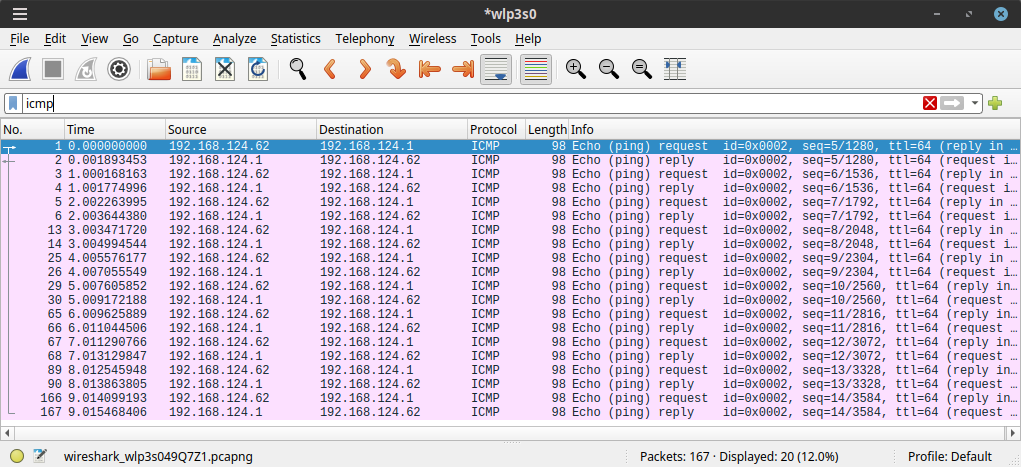
\includegraphics[scale=0.6]{res/5.wireshark-icmp.png}
\end{center}

Рассмотрим \texttt{ICMP} пакет, полученный в качестве эхо-ответа от удалённого хоста.

\subsection*{Канальный уровень (data link): Ethernet фрейм}
\addcontentsline{toc}{subsection}{Канальный уровень (data link): Ethernet фрейм}

Первые 6 байт -- MAC-адрес получателя пакета (\texttt{14:5a:fc:0d:56:2d}).

\fbox{
    \parbox{\textwidth}{%
    \texttt{\noindent
0000|   \hl{14 5a fc 0d 56 2d} 34 ce 00 37 d9 03 08 00 45 00\\
0010|   00 54 20 30 00 00 40 01 e0 e8 c0 a8 7c 01 c0 a8\\
0020|   7c 3e 00 00 d3 bd 00 02 00 0e 7a c1 e8 63 00 00\\
0030|   00 00 08 3a 02 00 00 00 00 00 10 11 12 13 14 15\\
0040|   16 17 18 19 1a 1b 1c 1d 1e 1f 20 21 22 23 24 25\\
0050|   26 27 28 29 2a 2b 2c 2d 2e 2f 30 31 32 33 34 35\\
0060|   36 37
    }}%
}

Следующие 6 байт -- MAC-адрес отправителя пакета (\texttt{34:ce:00:37:d9:03}).

\fbox{
    \parbox{\textwidth}{%
    \texttt{\noindent
0000|   14 5a fc 0d 56 2d \hl{34 ce 00 37 d9 03} 08 00 45 00\\
0010|   00 54 20 30 00 00 40 01 e0 e8 c0 a8 7c 01 c0 a8\\
0020|   7c 3e 00 00 d3 bd 00 02 00 0e 7a c1 e8 63 00 00\\
0030|   00 00 08 3a 02 00 00 00 00 00 10 11 12 13 14 15\\
0040|   16 17 18 19 1a 1b 1c 1d 1e 1f 20 21 22 23 24 25\\
0050|   26 27 28 29 2a 2b 2c 2d 2e 2f 30 31 32 33 34 35\\
0060|   36 37
    }}%
}

Тип пакетов -- IPv4 (\texttt{0x0800}). Полный список типов в удобном виде можно посмотреть в Wikipedia:\\\url{https://en.wikipedia.org/wiki/EtherType}

\fbox{
    \parbox{\textwidth}{%
    \texttt{\noindent
0000|   14 5a fc 0d 56 2d 34 ce 00 37 d9 03 \hl{08 00} 45 00\\
0010|   00 54 20 30 00 00 40 01 e0 e8 c0 a8 7c 01 c0 a8\\
0020|   7c 3e 00 00 d3 bd 00 02 00 0e 7a c1 e8 63 00 00\\
0030|   00 00 08 3a 02 00 00 00 00 00 10 11 12 13 14 15\\
0040|   16 17 18 19 1a 1b 1c 1d 1e 1f 20 21 22 23 24 25\\
0050|   26 27 28 29 2a 2b 2c 2d 2e 2f 30 31 32 33 34 35\\
0060|   36 37
    }}%
}

\subsection*{Сетевой уровень (network): IP пакет}
\addcontentsline{toc}{subsection}{Сетевой уровень (network): IP пакет}

Первые 4 бита указывают на версию IP. Код \texttt{0100} указывает на 4-ю версию. Структуру IPv4 пакета можно посмотреть в Wikipedia:\\\url{https://en.wikipedia.org/wiki/Internet_Protocol_version_4}

Следующие 4 бита передают длину хедера пакета. Код \texttt{0101} соответствует длинне в 20 байт.

\texttt{wireshark} показывает байт целиком.

\fbox{
    \parbox{\textwidth}{%
    \texttt{\noindent
0000|   14 5a fc 0d 56 2d 34 ce 00 37 d9 03 08 00 \hl{45} 00\\
0010|   00 54 20 30 00 00 40 01 e0 e8 c0 a8 7c 01 c0 a8\\
0020|   7c 3e 00 00 d3 bd 00 02 00 0e 7a c1 e8 63 00 00\\
0030|   00 00 08 3a 02 00 00 00 00 00 10 11 12 13 14 15\\
0040|   16 17 18 19 1a 1b 1c 1d 1e 1f 20 21 22 23 24 25\\
0050|   26 27 28 29 2a 2b 2c 2d 2e 2f 30 31 32 33 34 35\\
0060|   36 37
    }}%
}

Дальше идут сервисные поля \texttt{DSCP} (разделения трафика на классы обслуживания) и \texttt{ECN} (предупреждение о перегрузке сети без потери пакетов), в суть которых мы не будем углубляться, т.к. они всё равно не используются в данном случа.

\fbox{
    \parbox{\textwidth}{%
    \texttt{\noindent
0000|   14 5a fc 0d 56 2d 34 ce 00 37 d9 03 08 00 45 \hl{00}\\
0010|   00 54 20 30 00 00 40 01 e0 e8 c0 a8 7c 01 c0 a8\\
0020|   7c 3e 00 00 d3 bd 00 02 00 0e 7a c1 e8 63 00 00\\
0030|   00 00 08 3a 02 00 00 00 00 00 10 11 12 13 14 15\\
0040|   16 17 18 19 1a 1b 1c 1d 1e 1f 20 21 22 23 24 25\\
0050|   26 27 28 29 2a 2b 2c 2d 2e 2f 30 31 32 33 34 35\\
0060|   36 37
    }}%
}

Следующие 16 бит это полный размер пакета в байтах, включая заголовок и данные. По RFC, он может быть от 20 до 65535 байт. А нашем случае -- 84.

\fbox{
    \parbox{\textwidth}{%
    \texttt{\noindent
0000|   14 5a fc 0d 56 2d 34 ce 00 37 d9 03 08 00 45 00\\
0010|   \hl{00 54} 20 30 00 00 40 01 e0 e8 c0 a8 7c 01 c0 a8\\
0020|   7c 3e 00 00 d3 bd 00 02 00 0e 7a c1 e8 63 00 00\\
0030|   00 00 08 3a 02 00 00 00 00 00 10 11 12 13 14 15\\
0040|   16 17 18 19 1a 1b 1c 1d 1e 1f 20 21 22 23 24 25\\
0050|   26 27 28 29 2a 2b 2c 2d 2e 2f 30 31 32 33 34 35\\
0060|   36 37
    }}%
}

Далее идёт уникальный идентификатор, используемый для идентификации фрагментов пакета, если он был фрагментирован.

\fbox{
    \parbox{\textwidth}{%
    \texttt{\noindent
0000|   14 5a fc 0d 56 2d 34 ce 00 37 d9 03 08 00 45 00\\
0010|   00 54 \hl{20 30} 00 00 40 01 e0 e8 c0 a8 7c 01 c0 a8\\
0020|   7c 3e 00 00 d3 bd 00 02 00 0e 7a c1 e8 63 00 00\\
0030|   00 00 08 3a 02 00 00 00 00 00 10 11 12 13 14 15\\
0040|   16 17 18 19 1a 1b 1c 1d 1e 1f 20 21 22 23 24 25\\
0050|   26 27 28 29 2a 2b 2c 2d 2e 2f 30 31 32 33 34 35\\
0060|   36 37
    }}%
}

Следующие три бита -- поле флагов. Биты, от старшего к младшему, означают:
\begin{itemize}
    \item 0: Зарезервирован, должен быть равен 0
    \item 1: Не фрагментировать
    \item 2: У пакета ещё есть фрагменты
\end{itemize}

И после этого ещё 13 бит для указания смещение поля данных текущего фрагмента относительно начала поля данных первого фрагментированного пакета в блоках по 8 байт.

\fbox{
    \parbox{\textwidth}{%
    \texttt{\noindent
0000|   14 5a fc 0d 56 2d 34 ce 00 37 d9 03 08 00 45 00\\
0010|   00 54 20 30 \hl{00 00} 40 01 e0 e8 c0 a8 7c 01 c0 a8\\
0020|   7c 3e 00 00 d3 bd 00 02 00 0e 7a c1 e8 63 00 00\\
0030|   00 00 08 3a 02 00 00 00 00 00 10 11 12 13 14 15\\
0040|   16 17 18 19 1a 1b 1c 1d 1e 1f 20 21 22 23 24 25\\
0050|   26 27 28 29 2a 2b 2c 2d 2e 2f 30 31 32 33 34 35\\
0060|   36 37
    }}%
}

Время жизни пакета (Time to Live) задаёт максимальное количество маршрутизаторов (хопов) на пути следования пакета. Максимальное значение TTL=255, но чаще встречается TTL=64.

\fbox{
    \parbox{\textwidth}{%
    \texttt{\noindent
0000|   14 5a fc 0d 56 2d 34 ce 00 37 d9 03 08 00 45 00\\
0010|   00 54 20 30 00 00 \hl{40} 01 e0 e8 c0 a8 7c 01 c0 a8\\
0020|   7c 3e 00 00 d3 bd 00 02 00 0e 7a c1 e8 63 00 00\\
0030|   00 00 08 3a 02 00 00 00 00 00 10 11 12 13 14 15\\
0040|   16 17 18 19 1a 1b 1c 1d 1e 1f 20 21 22 23 24 25\\
0050|   26 27 28 29 2a 2b 2c 2d 2e 2f 30 31 32 33 34 35\\
0060|   36 37
    }}%
}

Следующее поле показывает, данные какого протокола IP содержит пакет (к примеру, это может быть TCP). Список кодов можно посмотреть на сайте IANA:\\\url{https://www.iana.org/assignments/protocol-numbers/protocol-numbers.xml}

Код \texttt{01} соответствует ICMP.

\fbox{
    \parbox{\textwidth}{%
    \texttt{\noindent
0000|   14 5a fc 0d 56 2d 34 ce 00 37 d9 03 08 00 45 00\\
0010|   00 54 20 30 00 00 40 \hl{01} e0 e8 c0 a8 7c 01 c0 a8\\
0020|   7c 3e 00 00 d3 bd 00 02 00 0e 7a c1 e8 63 00 00\\
0030|   00 00 08 3a 02 00 00 00 00 00 10 11 12 13 14 15\\
0040|   16 17 18 19 1a 1b 1c 1d 1e 1f 20 21 22 23 24 25\\
0050|   26 27 28 29 2a 2b 2c 2d 2e 2f 30 31 32 33 34 35\\
0060|   36 37
    }}%
}

Контрольная сумма заголовка занимает следующие 2-байта и используемая для проверки целостности заголовка

\fbox{
    \parbox{\textwidth}{%
    \texttt{\noindent
0000|   14 5a fc 0d 56 2d 34 ce 00 37 d9 03 08 00 45 00\\
0010|   00 54 20 30 00 00 40 01 \hl{e0 e8} c0 a8 7c 01 c0 a8\\
0020|   7c 3e 00 00 d3 bd 00 02 00 0e 7a c1 e8 63 00 00\\
0030|   00 00 08 3a 02 00 00 00 00 00 10 11 12 13 14 15\\
0040|   16 17 18 19 1a 1b 1c 1d 1e 1f 20 21 22 23 24 25\\
0050|   26 27 28 29 2a 2b 2c 2d 2e 2f 30 31 32 33 34 35\\
0060|   36 37
    }}%
}

Далее 32-битный адрес отправителя пакета (Может не совпадать с настоящим адресом отправителя из-за трансляции адресов -- NAT)

\fbox{
    \parbox{\textwidth}{%
    \texttt{\noindent
0000|   14 5a fc 0d 56 2d 34 ce 00 37 d9 03 08 00 45 00\\
0010|   00 54 20 30 00 00 40 01 e0 e8 \hl{c0 a8 7c 01} c0 a8\\
0020|   7c 3e 00 00 d3 bd 00 02 00 0e 7a c1 e8 63 00 00\\
0030|   00 00 08 3a 02 00 00 00 00 00 10 11 12 13 14 15\\
0040|   16 17 18 19 1a 1b 1c 1d 1e 1f 20 21 22 23 24 25\\
0050|   26 27 28 29 2a 2b 2c 2d 2e 2f 30 31 32 33 34 35\\
0060|   36 37
    }}%
}

И 32-битный адрес получателя пакета (учитывая, что это \texttt{ICMP}-ответ, получателем будет хост, на котором запущен \texttt{ping}).

\fbox{
    \parbox{\textwidth}{%
    \texttt{\noindent
0000|   14 5a fc 0d 56 2d 34 ce 00 37 d9 03 08 00 45 00\\
0010|   00 54 20 30 00 00 40 01 e0 e8 c0 a8 7c 01 \hl{c0 a8}\\
0020|   \hl{7c 3e} 00 00 d3 bd 00 02 00 0e 7a c1 e8 63 00 00\\
0030|   00 00 08 3a 02 00 00 00 00 00 10 11 12 13 14 15\\
0040|   16 17 18 19 1a 1b 1c 1d 1e 1f 20 21 22 23 24 25\\
0050|   26 27 28 29 2a 2b 2c 2d 2e 2f 30 31 32 33 34 35\\
0060|   36 37
    }}%
}

\subsection*{Сетевой уровень (network): ICMP пакет}
\addcontentsline{toc}{subsection}{Сетевой уровень (network): ICMP пакет}

Первый байт указывает на тип пакета.

Код \texttt{0} соответствует \texttt{ICMP}-ответу. Список кодов и заголовков можно посмотреть в Wikipedia:\\\url{https://en.wikipedia.org/wiki/Internet_Control_Message_Protocol}

\fbox{
    \parbox{\textwidth}{%
    \texttt{\noindent
0000|   14 5a fc 0d 56 2d 34 ce 00 37 d9 03 08 00 45 00\\
0010|   00 54 20 30 00 00 40 01 e0 e8 c0 a8 7c 01 c0 a8\\
0020|   7c 3e \hl{00} 00 d3 bd 00 02 00 0e 7a c1 e8 63 00 00\\
0030|   00 00 08 3a 02 00 00 00 00 00 10 11 12 13 14 15\\
0040|   16 17 18 19 1a 1b 1c 1d 1e 1f 20 21 22 23 24 25\\
0050|   26 27 28 29 2a 2b 2c 2d 2e 2f 30 31 32 33 34 35\\
0060|   36 37
    }}%
}

Следующий байт -- код, который зависит от типа пакета. Для \texttt{ICMP}-ответа возможно только 0-е значение.

\fbox{
    \parbox{\textwidth}{%
    \texttt{\noindent
0000|   14 5a fc 0d 56 2d 34 ce 00 37 d9 03 08 00 45 00\\
0010|   00 54 20 30 00 00 40 01 e0 e8 c0 a8 7c 01 c0 a8\\
0020|   7c 3e 00 \hl{00} d3 bd 00 02 00 0e 7a c1 e8 63 00 00\\
0030|   00 00 08 3a 02 00 00 00 00 00 10 11 12 13 14 15\\
0040|   16 17 18 19 1a 1b 1c 1d 1e 1f 20 21 22 23 24 25\\
0050|   26 27 28 29 2a 2b 2c 2d 2e 2f 30 31 32 33 34 35\\
0060|   36 37
    }}%
}

Ещё два байта нужны для передачи контрльной суммы.

\fbox{
    \parbox{\textwidth}{%
    \texttt{\noindent
0000|   14 5a fc 0d 56 2d 34 ce 00 37 d9 03 08 00 45 00\\
0010|   00 54 20 30 00 00 40 01 e0 e8 c0 a8 7c 01 c0 a8\\
0020|   7c 3e 00 00 \hl{d3 bd} 00 02 00 0e 7a c1 e8 63 00 00\\
0030|   00 00 08 3a 02 00 00 00 00 00 10 11 12 13 14 15\\
0040|   16 17 18 19 1a 1b 1c 1d 1e 1f 20 21 22 23 24 25\\
0050|   26 27 28 29 2a 2b 2c 2d 2e 2f 30 31 32 33 34 35\\
0060|   36 37
    }}%
}

Следующие 4 байта так же зависят от типа и кода.

\fbox{
    \parbox{\textwidth}{%
    \texttt{\noindent
0000|   14 5a fc 0d 56 2d 34 ce 00 37 d9 03 08 00 45 00\\
0010|   00 54 20 30 00 00 40 01 e0 e8 c0 a8 7c 01 c0 a8\\
0020|   7c 3e 00 00 d3 bd \hl{00 02 00 0e} 7a c1 e8 63 00 00\\
0030|   00 00 08 3a 02 00 00 00 00 00 10 11 12 13 14 15\\
0040|   16 17 18 19 1a 1b 1c 1d 1e 1f 20 21 22 23 24 25\\
0050|   26 27 28 29 2a 2b 2c 2d 2e 2f 30 31 32 33 34 35\\
0060|   36 37
    }}%
}

Далее идёт временная метка, для расчёта задержки при доставке сообщения

\fbox{
    \parbox{\textwidth}{%
    \texttt{\noindent
0000|   14 5a fc 0d 56 2d 34 ce 00 37 d9 03 08 00 45 00\\
0010|   00 54 20 30 00 00 40 01 e0 e8 c0 a8 7c 01 c0 a8\\
0020|   7c 3e 00 00 d3 bd 00 02 00 0e \hl{7a c1 e8 63 00 00}\\
0030|   \hl{00 00} 08 3a 02 00 00 00 00 00 10 11 12 13 14 15\\
0040|   16 17 18 19 1a 1b 1c 1d 1e 1f 20 21 22 23 24 25\\
0050|   26 27 28 29 2a 2b 2c 2d 2e 2f 30 31 32 33 34 35\\
0060|   36 37
    }}%
}

Оставшиеся 48 байт присылают в содержат тело запроса, полученное \texttt{ICMP}-сервером (по этой причине схема и получила название "эхо").

\fbox{
    \parbox{\textwidth}{%
    \texttt{\noindent
0000|   14 5a fc 0d 56 2d 34 ce 00 37 d9 03 08 00 45 00\\
0010|   00 54 20 30 00 00 40 01 e0 e8 c0 a8 7c 01 c0 a8\\
0020|   7c 3e 00 00 d3 bd 00 02 00 0e 7a c1 e8 63 00 00\\
0030|   00 00 \hl{08 3a 02 00 00 00 00 00 10 11 12 13 14 15}\\
0040|   \hl{16 17 18 19 1a 1b 1c 1d 1e 1f 20 21 22 23 24 25}\\
0050|   \hl{26 27 28 29 2a 2b 2c 2d 2e 2f 30 31 32 33 34 35}\\
0060|   \hl{36 37}
    }}%
}

Значения для полей при различных режимах работы \texttt{ICMP} приведены в Wikipedia:\\\url{https://en.wikipedia.org/wiki/Internet_Control_Message_Protocol}

\section*{3. Анализ ARP трафика}
\addcontentsline{toc}{section}{3. Анализ ARP трафика}

Протокол разрешения адресов (\texttt{Address Resolution Protocol}, \texttt{ARP}) используется в компьютерных сетях для сопоставления \texttt{IP}-адресов и \texttt{MAC}-адресов в рамках одного широковещательного домена. Механизм сопоставления называют "\texttt{ARP}-таблицами" и этот механизм подвержен различными атакам (типа переполнения размерности) для встраивания в цепочку передачи (\texttt{Man-in-the-middle}).

Отображение \texttt{ARP}-таблицы на беспроводном интерфейсе
\begin{Verbatim}[frame=single,breaklines=true,breakanywhere=true]
    smart@thinkpad$ ip neigh show dev wlp3s0
    192.168.124.1 lladdr 34:ce:00:37:d9:03 REACHABLE 
    fe80::36ce:ff:fe37:d903 lladdr 34:ce:00:37:d9:03 router REACHABLE 
\end{Verbatim}

Фильтрация \texttt{ARP} пакетов в \texttt{wireshark}
\begin{center}
    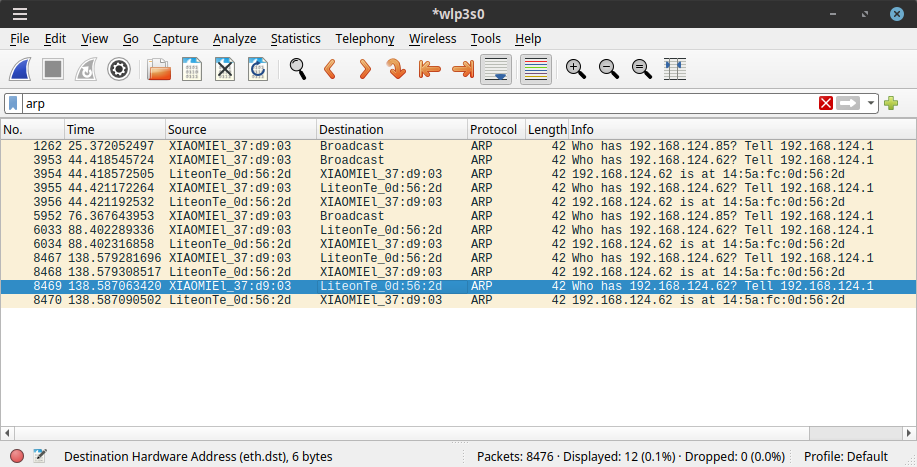
\includegraphics[scale=0.6]{res/5.wireshark-arp.png}
\end{center}

\subsection*{Канальный уровень (data link): Ethernet фрейм}
\addcontentsline{toc}{subsection}{Канальный уровень (data link): Ethernet фрейм}

\texttt{MAC}-адрес получателя \texttt{ff:ff:ff:ff:ff:ff}. Широковещательное (Broadcast) сообщение.

\fbox{
    \parbox{\textwidth}{%
    \texttt{\noindent
0000|   \hl{ff ff ff ff ff ff} 34 ce 00 37 d9 03 08 06 00 01\\
0010|   08 00 06 04 00 01 34 ce 00 37 d9 03 c0 a8 7c 01\\
0020|   00 00 00 00 00 00 c0 a8 7c 55
    }}%
}

\texttt{MAC}-адрес отправителя \texttt{34:ce:00:37:d9:03}

\fbox{
    \parbox{\textwidth}{%
    \texttt{\noindent
0000|   ff ff ff ff ff ff \hl{34 ce 00 37 d9 03} 08 06 00 01\\
0010|   08 00 06 04 00 01 34 ce 00 37 d9 03 c0 a8 7c 01\\
0020|   00 00 00 00 00 00 c0 a8 7c 55
    }}%
}

Тип сообщения -- \texttt{ARP} (\texttt{0x0806}). Справочник в Wikipedia:\\\url{https://en.wikipedia.org/wiki/EtherType}

\fbox{
    \parbox{\textwidth}{%
    \texttt{\noindent
0000|   ff ff ff ff ff ff 34 ce 00 37 d9 03 \hl{08 06} 00 01\\
0010|   08 00 06 04 00 01 34 ce 00 37 d9 03 c0 a8 7c 01\\
0020|   00 00 00 00 00 00 c0 a8 7c 55
    }}%
}

\subsection*{Сетевой уровень (network): ARP пакет}
\addcontentsline{toc}{subsection}{Сетевой уровень (network): ARP пакет}

Структура пакетов и значения флагов описаны в Wikipedia:\\\url{https://ru.wikipedia.org/wiki/ARP}

Первые два байта -- тип канального протокола. \texttt{Ethernet} имеет номер \texttt{0x0001}.

\fbox{
    \parbox{\textwidth}{%
    \texttt{\noindent
0000|   ff ff ff ff ff ff 34 ce 00 37 d9 03 08 06 \hl{00 01}\\
0010|   08 00 06 04 00 01 34 ce 00 37 d9 03 c0 a8 7c 01\\
0020|   00 00 00 00 00 00 c0 a8 7c 55
    }}%
}

Ещё два байта для кода сетевого протокола. Для \texttt{IPv4} код \texttt{0x0800}.

\fbox{
    \parbox{\textwidth}{%
    \texttt{\noindent
0000|   ff ff ff ff ff ff 34 ce 00 37 d9 03 08 06 00 01\\
0010|   \hl{08 00} 06 04 00 01 34 ce 00 37 d9 03 c0 a8 7c 01\\
0020|   00 00 00 00 00 00 c0 a8 7c 55
    }}%
}

Длина физического адреса в байтах. Адреса \texttt{Ethernet} имеют длину 6 байт (\texttt{0x06})

\fbox{
    \parbox{\textwidth}{%
    \texttt{\noindent
0000|   ff ff ff ff ff ff 34 ce 00 37 d9 03 08 06 00 01\\
0010|   08 00 \hl{06} 04 00 01 34 ce 00 37 d9 03 c0 a8 7c 01\\
0020|   00 00 00 00 00 00 c0 a8 7c 55
    }}%
}

Длина логического адреса в байтах. \texttt{IPv4} адреса имеют длину 4 байта (\texttt{0x04}).

\fbox{
    \parbox{\textwidth}{%
    \texttt{\noindent
0000|   ff ff ff ff ff ff 34 ce 00 37 d9 03 08 06 00 01\\
0010|   08 00 06 \hl{04} 00 01 34 ce 00 37 d9 03 c0 a8 7c 01\\
0020|   00 00 00 00 00 00 c0 a8 7c 55
    }}%
}

Код операции отправителя: \texttt{0x0001} в случае запроса и \texttt{0x0002} в случае ответа.

\fbox{
    \parbox{\textwidth}{%
    \texttt{\noindent
0000|   ff ff ff ff ff ff 34 ce 00 37 d9 03 08 06 00 01\\
0010|   08 00 06 04 \hl{00 01} 34 ce 00 37 d9 03 c0 a8 7c 01\\
0020|   00 00 00 00 00 00 c0 a8 7c 55
    }}%
}

Физический адрес отправителя (SHA)

\fbox{
    \parbox{\textwidth}{%
    \texttt{\noindent
0000|   ff ff ff ff ff ff 34 ce 00 37 d9 03 08 06 00 01\\
0010|   08 00 06 04 00 01 \hl{34 ce 00 37 d9 03} c0 a8 7c 01\\
0020|   00 00 00 00 00 00 c0 a8 7c 55
    }}%
}

Логический адрес отправителя (SPA)

\fbox{
    \parbox{\textwidth}{%
    \texttt{\noindent
0000|   ff ff ff ff ff ff 34 ce 00 37 d9 03 08 06 00 01\\
0010|   08 00 06 04 00 01 34 ce 00 37 d9 03 \hl{c0 a8 7c 01}\\
0020|   00 00 00 00 00 00 c0 a8 7c 55
    }}%
}

Физический адрес получателя (THA). Не требуется при запросе.

\fbox{
    \parbox{\textwidth}{%
    \texttt{\noindent
0000|   ff ff ff ff ff ff 34 ce 00 37 d9 03 08 06 00 01\\
0010|   08 00 06 04 00 01 34 ce 00 37 d9 03 c0 a8 7c 01\\
0020|   \hl{00 00 00 00 00 00} c0 a8 7c 55
    }}%
}

Логический адрес получателя(TPA).

\fbox{
    \parbox{\textwidth}{%
    \texttt{\noindent
0000|   ff ff ff ff ff ff 34 ce 00 37 d9 03 08 06 00 01\\
0010|   08 00 06 04 00 01 34 ce 00 37 d9 03 c0 a8 7c 01\\
0020|   00 00 00 00 00 00 \hl{c0 a8 7c 55}
    }}%
}

\section*{3. Анализ FTP трафика}
\addcontentsline{toc}{section}{3. Анализ FTP трафика}

Для работы с FTP, используем проект \texttt{vsftpd} (very secure FTP daemon).

Так же создадим виртуальный сервер с публичным \texttt{IP} адресом и присвоим ему доменное имя (это понадобится в будущем для получения \texttt{TLS}-сертификатов).

\subsection*{Демонстрация уязвимости}
\addcontentsline{toc}{subsection}{Демонстрация уязвимости}

Осуществим запуск \texttt{vsftd} в docker-контейнере. Имя пользователя \texttt{one}, пароль \texttt{1234}.
\begin{Verbatim}[frame=single,breaklines=true,breakanywhere=true]
    ubuntu@temp$ docker run -d \
        -p 21:21 \
        -p 21000-21010:21000-21010 \
        -e USERS="one|1234" \
        -e ADDRESS=ftp.deeprosoft.com \
        delfer/alpine-ftp-server
    Unable to find image 'delfer/alpine-ftp-server:latest' locally
    latest: Pulling from delfer/alpine-ftp-server
    df9b9388f04a: Pull complete 
    dff9a38fdd78: Pull complete 
    961dffff6741: Pull complete 
    99d694c3fc07: Pull complete 
    2dbb22f0414d: Pull complete 
    Digest: sha256:b030e5ee82965fb7d7135f8dbffd77c9b753ef1b60d22d1f4eb92d4d37f71c13
    Status: Downloaded newer image for delfer/alpine-ftp-server:latest
    a188e56c28dca2e19e517960b2ae526c306147d24fa364471368f79debd75e08
\end{Verbatim}

FTP является устаревшим протоколом, и его поддержка давно удалена из браузеров. По этой причине необходимо явным образом установить FTP-клиент.
\begin{Verbatim}[frame=single,breaklines=true,breakanywhere=true]
    smart@thinkpad$ sudo pacman -S filezilla
    [sudo] password for smart: 
    resolving dependencies...
    looking for conflicting packages...

    Packages (2) libfilezilla-1:0.41.0-1  filezilla-3.63.1-1

    Total Download Size:    4.69 MiB
    Total Installed Size:  17.54 MiB

    :: Proceed with installation? [Y/n] 
    :: Retrieving packages...
    libfilezilla-1:0...   405.5 KiB  1179 KiB/s 00:00 [######################] 100%
    filezilla-3.63.1...     4.3 MiB  4.63 MiB/s 00:01 [######################] 100%
    Total (2/2)             4.7 MiB  4.81 MiB/s 00:01 [######################] 100%
    (2/2) checking keys in keyring                     [######################] 100%
    (2/2) checking package integrity                   [######################] 100%
    (2/2) loading package files                        [######################] 100%
    (2/2) checking for file conflicts                  [######################] 100%
    (2/2) checking available disk space                [######################] 100%
    :: Processing package changes...
    (1/2) installing libfilezilla                      [######################] 100%
    (2/2) installing filezilla                         [######################] 100%
    :: Running post-transaction hooks...
    (1/3) Arming ConditionNeedsUpdate...
    (2/3) Updating icon theme caches...
    (3/3) Updating the desktop file MIME type cache...
\end{Verbatim}

Ещё на стадии подключения, \texttt{filezilla} предупреждает о небезопасности подобного подключения
\begin{center}
    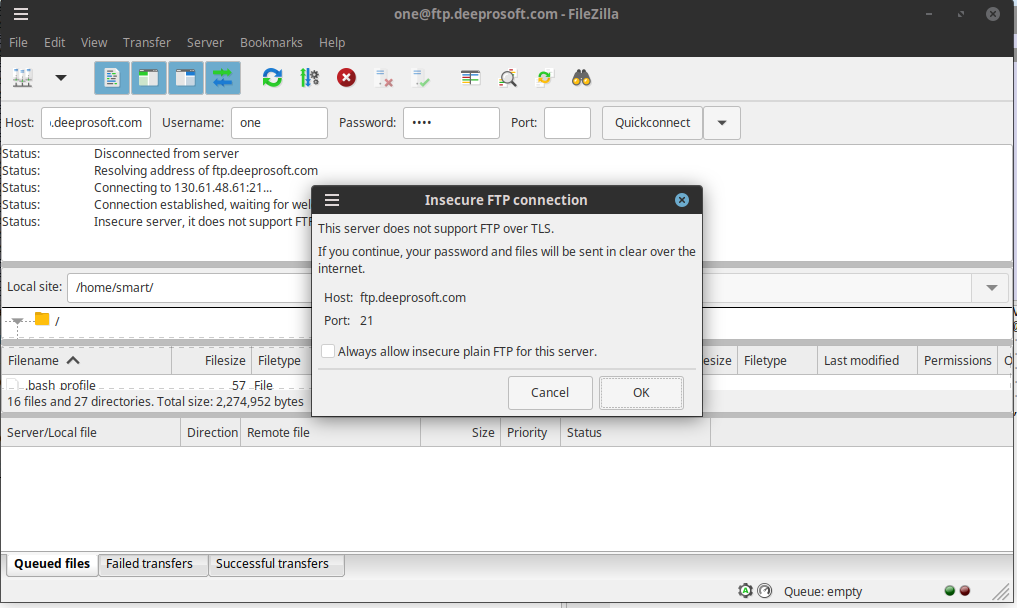
\includegraphics[scale=0.5]{res/5.filezilla-warning.png}
\end{center}

\newpage

При анализе трафика в \texttt{wireshark}, мы видим что со стороны \texttt{filezilla} была попытка установить соединение с использованием \texttt{TLS} и \texttt{SSL}, и только после этого имя пользователя и пароль были переданы в виде чистого текста.
\begin{center}
    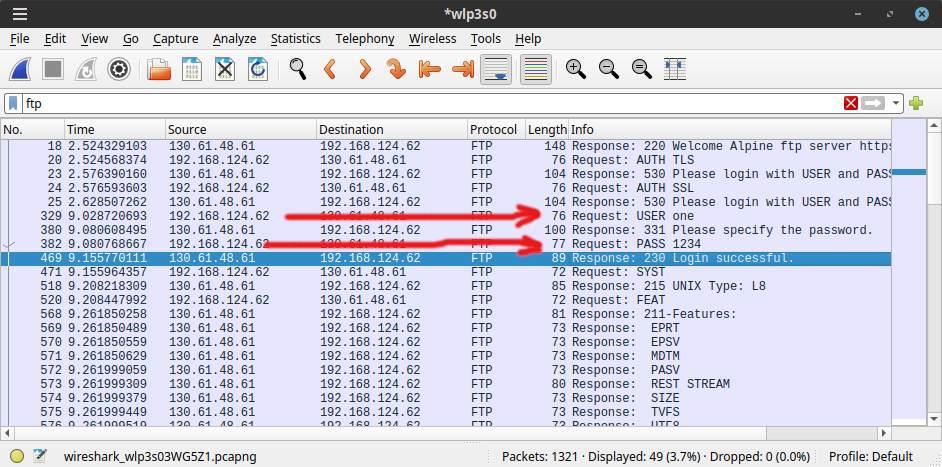
\includegraphics[scale=0.55]{res/5.wireshark-ftp-plain.png}
\end{center}

\subsection*{Шифровние трафика}
\addcontentsline{toc}{subsection}{Шифровние трафика}

Никакие изменения настроек (смена банеров приветствия, отключение анонимного доступа) \texttt{vsftd} не решит проблему передачи логина и пароля в чистом виде. Необходимо организовать обеспечить шифрование канала, а для этого нужно использовать валидные TLS-сертификаты (воспользуемся службой \texttt{LetsEncrypt}).

\begin{Verbatim}[frame=single,breaklines=true,breakanywhere=true]
    ubuntu@temp$ docker run -it --rm \
        -p 80:80 \
        -v "/etc/letsencrypt:/etc/letsencrypt" \
        certbot/certbot certonly \
        --standalone \
        --preferred-challenges http \
        -n --agree-tos \
        --email martynov.sa@edu.spbstu.ru \
        -d ftp.deeprosoft.com
    Unable to find image 'certbot/certbot:latest' locally
    latest: Pulling from certbot/certbot
    ca7dd9ec2225: Pull complete 
    9e124a36b9ab: Pull complete 
    42cba90def7f: Pull complete 
    036c0ab6a768: Pull complete 
    de6312618cf7: Pull complete 
    f2b159e8e18d: Pull complete 
    5c3094a661e9: Pull complete 
    ae4269d8cd1f: Pull complete 
    fc17a613a054: Pull complete 
    7560c853872e: Pull complete 
    ab060fadf2d2: Pull complete 
    b81696353590: Pull complete 
    144b4c29fbe6: Pull complete 
    Digest: sha256:f632e55104da84ba5b54bc858a67ac6c9b4f68790ea823515867c993153c3fb4
    Status: Downloaded newer image for certbot/certbot:latest
    Saving debug log to /var/log/letsencrypt/letsencrypt.log
    Account registered.
    Requesting a certificate for ftp.deeprosoft.com

    Successfully received certificate.
    Certificate is saved at: /etc/letsencrypt/live/ftp.deeprosoft.com/fullchain.pem
    Key is saved at:         /etc/letsencrypt/live/ftp.deeprosoft.com/privkey.pem
    This certificate expires on 2023-05-13.
    These files will be updated when the certificate renews.

    NEXT STEPS:
    - The certificate will need to be renewed before it expires. Certbot can automatically renew the certificate in the background, but you may need to take steps to enable that functionality. See https://certbot.org/renewal-setup for instructions.

    - - - - - - - - - - - - - - - - - - - - - - - - - - - - - - - - - - - - - - - -
    If you like Certbot, please consider supporting our work by:
    * Donating to ISRG / Let's Encrypt:   https://letsencrypt.org/donate
    * Donating to EFF:                    https://eff.org/donate-le
    - - - - - - - - - - - - - - - - - - - - - - - - - - - - - - - - - - - - - - - -
\end{Verbatim}

Теперь запустим \texttt{vsftd}, используя полученные \texttt{TLS}-сертификаты.

\begin{Verbatim}[frame=single,breaklines=true,breakanywhere=true]
    ubuntu@temp$ docker run -d \
        --name ftp \
        -v /etc/letsencrypt:/etc/letsencrypt:ro \
        -p 21:21 \
        -p 21000-21010:21000-21010 \
        -e USERS="one|1234" \
        -e ADDRESS=ftp.deeprosoft.com \
        -e TLS_CERT="/etc/letsencrypt/live/ftp.deeprosoft.com/fullchain.pem" \
        -e TLS_KEY="/etc/letsencrypt/live/ftp.deeprosoft.com/privkey.pem" \
        delfer/alpine-ftp-server
    02c57ccb66c3179da831927af6fe53c29a2ab59926e0901b0fb189ddbc66d06c
\end{Verbatim}

\newpage

Произведём подключение по протоколу \texttt{ftps}.
\begin{center}
    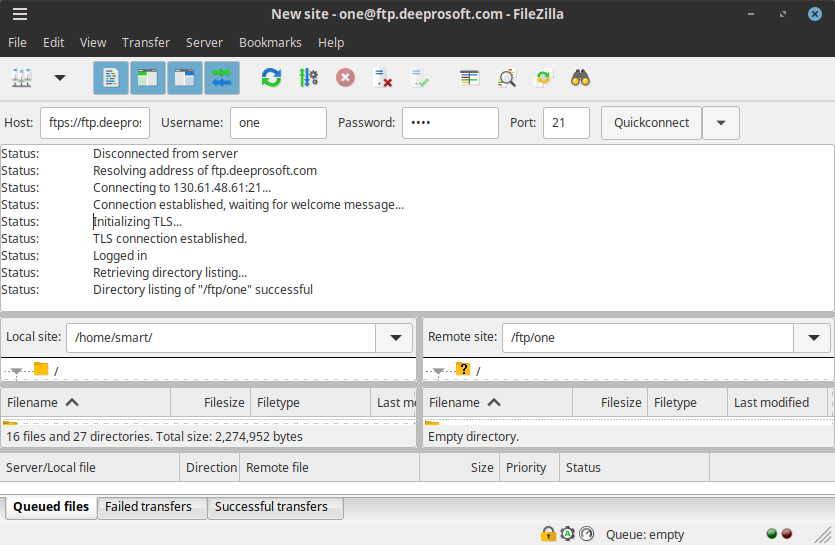
\includegraphics[scale=0.55]{res/5.filezilla-ftps.png}
\end{center}

Снифер \texttt{wireshark} уже не может перехватить пароль.
\begin{center}
    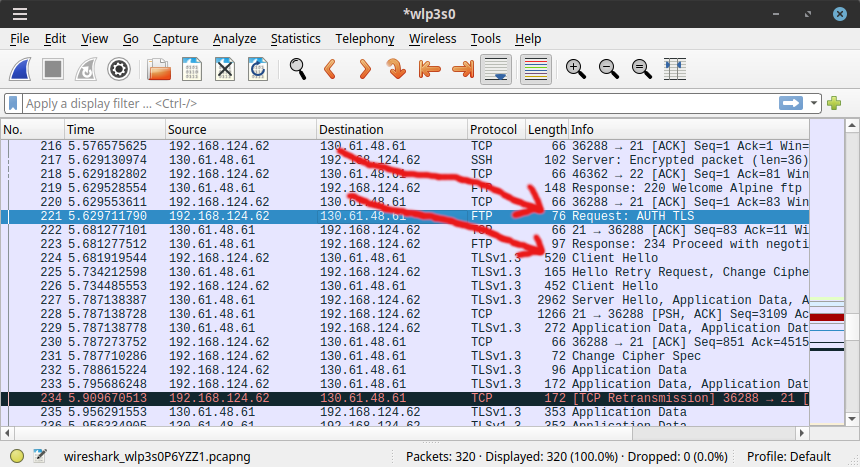
\includegraphics[scale=0.55]{res/5.wireshark-ftps.png}
\end{center}

\newpage

\section*{4. Сравнение защиты Telnet и SSH}
\addcontentsline{toc}{section}{4. Сравнение защиты Telnet и SSH}

Подготовим и запустим \texttt{Telnet} сервер в \texttt{Docker} окружении.
\begin{Verbatim}[frame=single,breaklines=true,breakanywhere=true]
    smart@thinkpad$ docker run -itd -p 23:23 --name=telnetServer flemingcsi/telnet-server
    Unable to find image 'flemingcsi/telnet-server:latest' locally
    latest: Pulling from flemingcsi/telnet-server
    c3b9c0688e3b: Pull complete 
    e9fb5affebb0: Pull complete 
    0f1378f511ad: Pull complete 
    96a961dc7843: Pull complete 
    16564141bc83: Pull complete 
    13bab7266e87: Pull complete 
    Digest: sha256:d667ca1bf508945dffe1de37812bac96469041471f9a1831567cf54004c7e400
    Status: Downloaded newer image for flemingcsi/telnet-server:latest
    066114bb8b7fbb57985e5289bfedc17c5634ac8d9fb2ffaca75bac66b0e075e4
\end{Verbatim}

Уточняю, какой адрес у запущенного сервиса
\begin{Verbatim}[frame=single,breaklines=true,breakanywhere=true]
    smart@thinkpad$ docker inspect --format={{.NetworkSettings.IPAddress}} telnetServer
    172.17.0.2
\end{Verbatim}

Теперь можно воспользоваться \texttt{nc} в качестве \texttt{telnet}-клиента.

При подключении есть какие-то проблемы с кодировкой, но это не важно.

\begin{Verbatim}[frame=single,breaklines=true,breakanywhere=true]
    smart@thinkpad$ nc 127.14.0.2 23
    ???? ?????'username
    password
\end{Verbatim}

\newpage

Снифер \texttt{wireshark} легко перехватывает все сообщения.
\begin{center}
    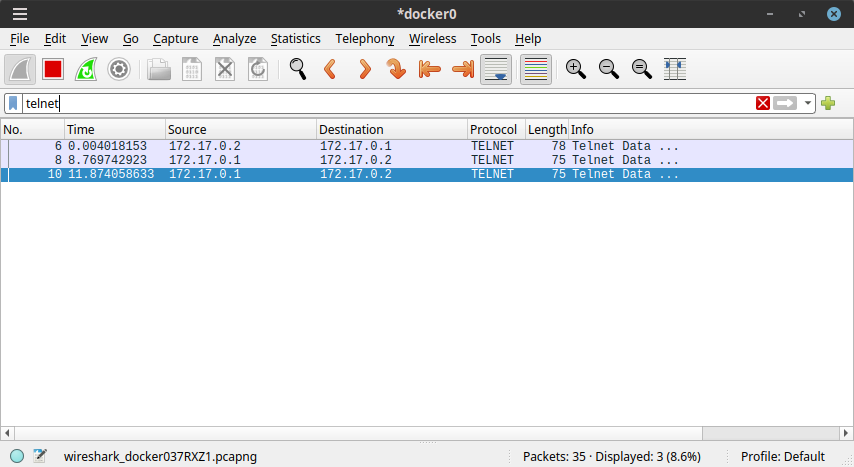
\includegraphics[scale=0.55]{res/5.wireshark-telnet.png}
\end{center}

В меню можно выбрать "Follow TCP stream" для более удобного прочтения перехваченных данных.

Можно без труда получить имя пользователя и пароль, можно просматривать все данные, передаваемые в обе стороны и даже подменять их на лету.

\begin{center}
    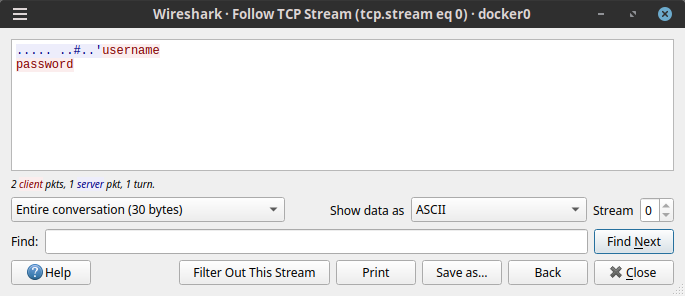
\includegraphics[scale=0.7]{res/5.wireshark-follow-stream.png}
\end{center}

\newpage

При подключении по \texttt{SSH} можно только увидеть \texttt{IP}-адреса клиента и сервера, а так же процесс согласования ключей на эллиптических кривых.

\begin{center}
    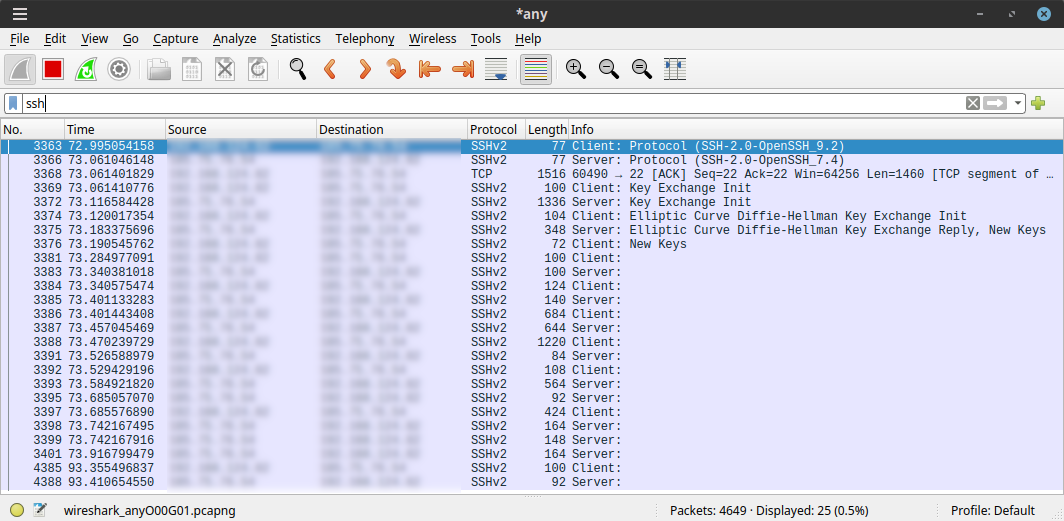
\includegraphics[scale=0.55]{res/5.wireshark-ssh.png}
\end{center}

Просмотреть какой-то трафик не получится, т.к. он надёжно шифруется.

\begin{center}
    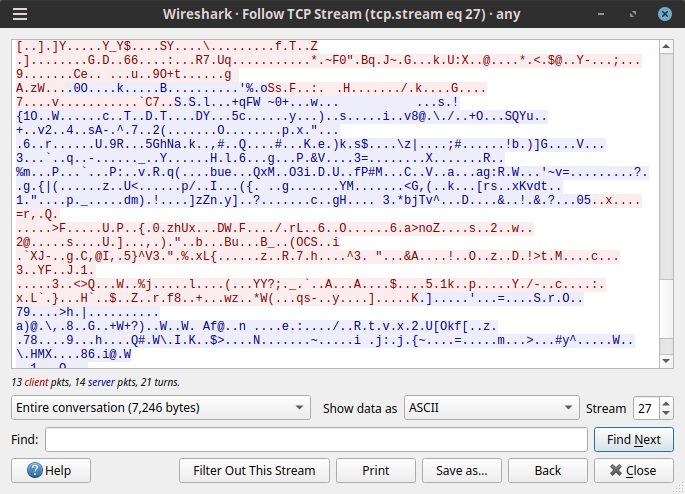
\includegraphics[scale=0.55]{res/5.wireshark-ssh-follow.png}
\end{center}


\section*{5. Анализ сообщений транспортного уровня: UDP-дейтаграммы и TCP-сегменты}
\addcontentsline{toc}{section}{5. Анализ сообщений транспортного уровня: UDP-дейтаграммы и TCP-сегменты}

Все различия происходят из архитектуры этих протоколов.

При фильтрации по \texttt{TCP}, особенно при интенсивном трафике, мы видем большое количество пакетов, связанных с исправлением различных ошибочных ситуаций. При фильтрации по \texttt{UDP} мы видим много пакетов, задача которых в нотификации.

\begin{center}
    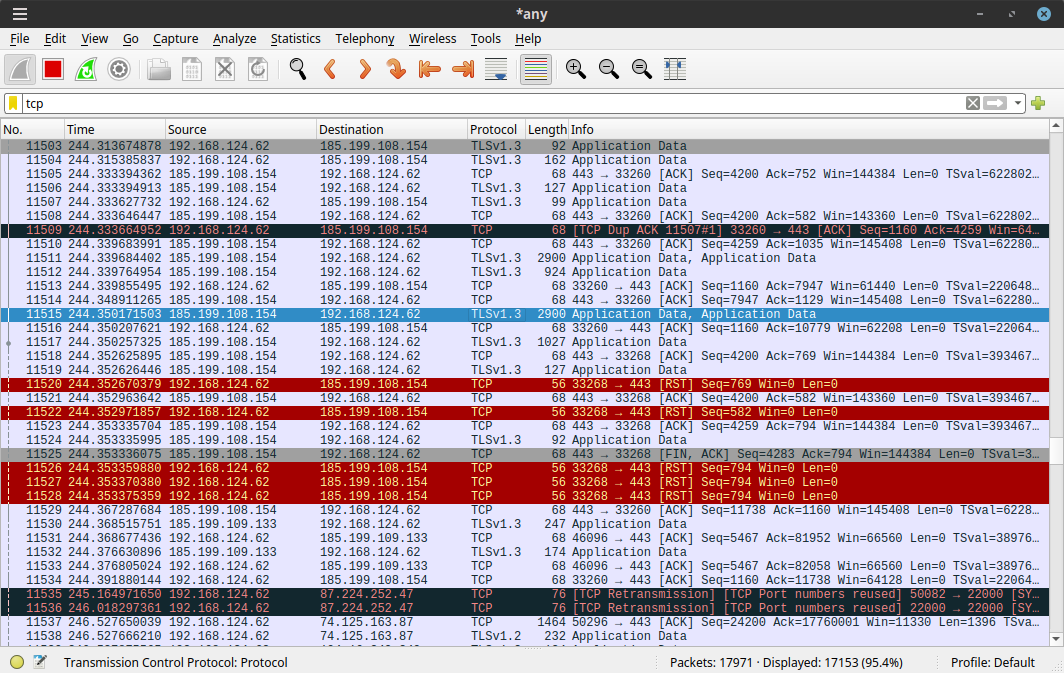
\includegraphics[scale=0.5]{res/5.wireshark-tcp.png}
\end{center}

В каждый пакет данных TCP добавляет заголовок общим объемом в 20 байт (или октетов), в котором содержатся 10 обязательных полей:
\begin{itemize}
    \item Порт источника -- порт устройства-отправителя.
    \item Порт назначения -- порт принимающего устройства.
    \item Порядковый номер -- Устройство, инициирующее TCP-соединение, должно выбрать случайный начальный порядковый номер, который затем увеличивается в соответствии с количеством переданных байтов.
    \item Номер подтверждения -- Принимающее устройство увеличивает этот номер с нуля в соответствии с количеством полученных байтов.
    \item Сдвиг данных TCP -- Данный параметр определяет размер заголовка, чтобы система могла понять, где начинаются данные.
    \item Зарезервированные данные -- зарезервированное поле, значение которого всегда равно нулю. 
    \item Флаги управления -- TCP использует девять флагов для управления потоком данных в определенных ситуациях (например, при инициировании сброса сессии).
    \item Контрольная сумма -- Отправитель генерирует контрольную сумму и передает ее в заголовке каждого пакета. Принимающее устройство может использовать контрольную сумму для проверки ошибок в полученном файле.
    \item Срочный указатель -- это предлагаемая протоколом возможность помечать некоторые байты данных тегом «Срочно» для их пересылки и обработки вне очереди.
    \item Поле опции -- Может использоваться для расширения протокола или его тестирования.
\end{itemize}

\begin{center}
    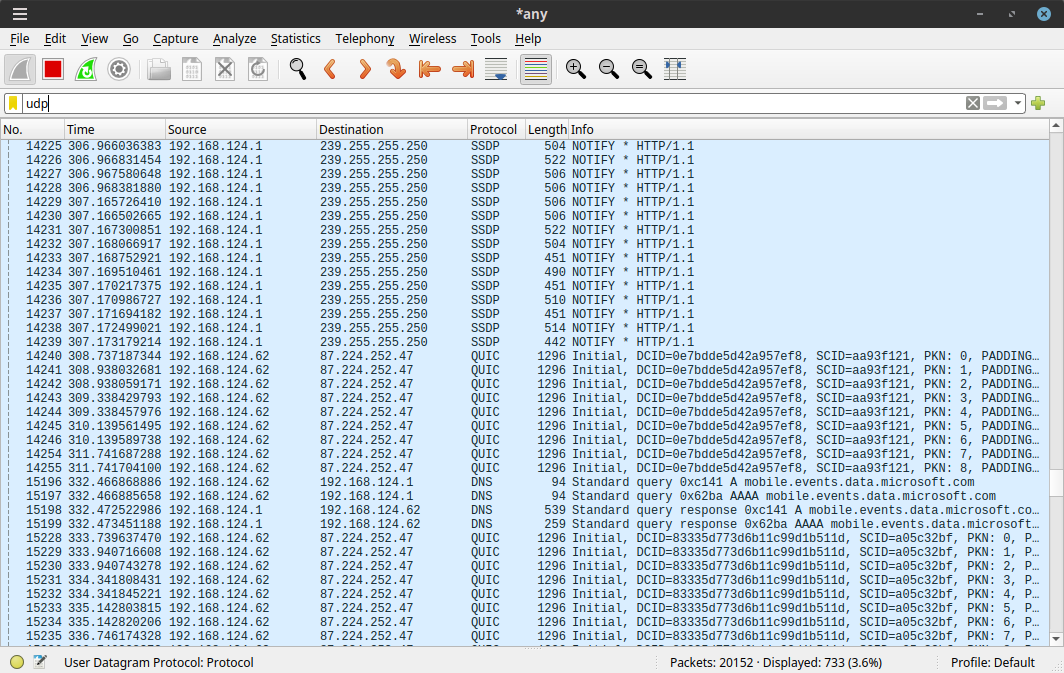
\includegraphics[scale=0.5]{res/5.wireshark-udp.png}
\end{center}

Заголовки UDP значительно проще.
\begin{itemize}
    \item Порт отправителя -- номер порта отправителя
    \item Порт получателя -- содержит порт получателя
    \item Длина датаграммы -- Поле, задающее длину всей датаграммы (заголовка и данных) в байтах. Минимальная длина равна длине заголовка -- 8 байт. Теоретически, максимальный размер поля -- 65535 байт для UDP-датаграммы (8 байт на заголовок и 65527 на данные).
\end{itemize}

\section*{Выводы}
\addcontentsline{toc}{section}{Выводы}

В реальной жизни достаточно тяжело встретиться с такими устаревшими протоколами как \texttt{FTP} или \texttt{Telnet}, но полезно знать об их уязвимостях. В процессе работы использовался сетевой снифер \texttt{wireshark}. На практике инженеры обычно используют \texttt{tcpdump}, но \texttt{wireshark} позволяет легко визуализировать трафик и разложить пакет по битам.

Так же было проведено сравнение между \texttt{TCP} и \texttt{UDP}. Ключевым различием между \texttt{TCP} и \texttt{UDP} является скорость, поскольку \texttt{TCP} сравнительно сложнее \texttt{UDP}. В целом, \texttt{UDP} является быстрым, простым и эффективным протоколом, однако повторная передача потерянных пакетов данных возможна только в \texttt{TCP}.